\section{Introduction}

% contextualizacao
Throughout the web, data is often presented in a semi-structured fashion (e.g.,
shopping items, news, search engine results, etc.) with the objective of
organizing semantically related entities in order to facilitate the
comprehension of the document by a human user. This semi-structured data,
although varied in layout and domain, has similar characteristics that can be
used to identify it inside a document and to improve its structure to the point
where it is possible to access it as relational data (i.e., as structured data).

% justificativa da importancia da pesquisa e motivacao
The extraction of structured information is undeniably both important and
difficult. It is an important task due to the ever growing amount of information
published and readily available on the web and because structured information
can be used to enrich, and allow, a number of applications (e.g., price
comparison, semantic keyword search, metasearch, etc.)
\cite{relationalWeb2008,kalyanpur2012structured,2015webtables}.
It is a difficult task because the data is laid out for human consumption and
published in a variety of formats and templates, as observed in
\cite{structured2011}. Moreover, the Beckman report on database
research\cite{abadi2014beckman} mentions the diversity of data as a key
challenge in this research field. The subset of structured data we address in
this work is a major data source according to \cite{structured2011}, since it
can be considered a generalization of the data addressed by WebTables
\cite{webtables2008}, we quote from \cite{structured2011}:
\begin{quote} 
``\textit{Hypertext-based data models}. These models, in which page authors use
combinations of HTML elements (such as a list of hyperlinks), perform certain 
data-model tasks (such as indicate that all entities pointed to by the
hyperlinks belong to the same set); this category can be considered a
\textbf{generalization} of the observation that HTML tables are used to
communicate relations;''
\end{quote}

% breve resumo bibliografico
Identifying the underlying content structure in a web document was attempted
before. The existing approaches range from solutions to specific instances of
the problem (e.g., extracting only data formatted with specific HTML
tags\cite{webtables2008,listExtract2009,qiu2015dexter}) to broader attempts that
search for patterns in a web
document\cite{MDR03,NET05,depta05,TPC09,grigalis2013towards}.
They also vary in degree of automation where there can be supervised,
semi-supervised and unsupervised approaches. It is our understanding that the
scientific community should strive to achieve the highest possible level of
automation when dealing with web extraction, due to the volume of data,
otherwise an eventual approach will not scale up. For this reason we will focus
on unsupervised approaches in this paper.
Existing work fails to definitively solve the problem, as observed in recent
surveys\cite{survey2013,survey2014}, they solve just a part of it. The ideal
solution should be unsupervised, computationally efficient, effective (at
least near perfect precision) and as general as possible (e.g., domain
independent and HTML syntax independent).

% resumo da abordagem
Here we outline a novel approach for the problem of structured extraction (or
record extraction) from web pages, using an alternative representation of the
DOM tree and some signal processing techniques. Our approach first converts the
DOM tree to a sequence representation; segments the sequence into regions;
identifies the regions with structured content; locates the records boundaries
within the structured regions and; aligns the records into a table. The
technique outlined here has the following characteristics: it takes a single
page as input, does not need training and it is unsupervised, computationally
efficient ($O(nlogn)$) and domain independent. It is also effective (we provide
a mechanism to ensure high precision at the expense of recall) and HTML syntax
independent, i.e., there are no heuristic rules targeted at specific tags.

% motivacao para uso de processamento de sinais
When the DOM tree is converted into its sequence representation, and plotted in
a graph, the patterns of structured data become evident (see Figure
\ref{fig:stru} for instance). That said, the research area concerned with signal
processing has been dealing with pattern detection and recognition long before
the web became what it is today (e.g., Fast Fourier Transform --
FFT\cite{fft1965} algorithm as published in 1965) and as a consequence it is
much more developed in that aspect, so it is only logical to employ some of
these consolidated techniques once we succeed converting the problem of
record extraction into a signal processing problem.

% detalhes do uso processamento de sinais
The adopted sequence representation enables the use of signal processing
techniques that, otherwise, would not be possible. The sequence is segmented
into cyclic subsequences, which represent structured data regions, using the
finite difference (Definition \ref{def:diff}). Within each of this cyclic
subsequences we use its spectrum (Definition \ref{def:fft}) to find their main
period (which represents the size of the records) and frequency (which
represents the number of records within that data region). Once we have the
main period (record size) and frequency (record count) we use this information
to break down the data region into records that are subsequently aligned.

% contribuicoes
The main contributions presented here are:
\begin{enumerate}
    \item a novel insight on how the structure of a web document can be seen: as
    a periodic signal. To the best of our knowledge there is nothing alike in
    the literature and the results depict both its efficiency and effectiveness;
    \item a novel web page segmentation technique;
    \item a new and efficient way of checking if a given region of a web page is
    structured or not. Such a framework, that is independent of the extraction
    process (i.e., one doesn't need to extract the entire document), is useful
    to avoid processing portions of the document that are unpromising be it for
    record extraction, clustering, indexing or any other end;
    \item a more efficient approach, when compared to the state-of-the-art,
    that is due to the use of efficient signal processing algorithms. Most
    existing works rely mainly on dynamic programming (e.g., edit distance), clustering
    algorithms and/or full page rendering and hence are less efficient.
\end{enumerate}

% organizacao do restante do texto
The rest of the paper is organized as follows. In Section \ref{sec:work} we
briefly review the work related to structured extraction; in Section
\ref{sec:defs} we presents some definitions required to better understand the
proposed approach for the problem; in Section \ref{sec:prop} we outline the
proposed approach; in Section \ref{sec:result} we discuss and compare the
achieved results and; in Section \ref{sec:con} we conclude and present some
of our ideas for future work.

\section{Related Work}\label{sec:work}

The task of extracting records from web pages has been approached from many
angles. Some authors proposed \textit{ad hoc} solutions while others tried 
broader approaches for the problem.

In \cite{webtables2008, listExtract2009, tablesMS2012, tegra2015, qiu2015dexter,
topklists2013} the records (or tables, for that matter) are extracted from very
specific sources like data formatted with \texttt{<table>},
\texttt{<ul/ol/etc.>} or even specific templates. Although these approaches may
seem to be limited, at least at a first glance, they actually yield sound
results as documented in \cite{relationalWeb2008, probase, probase2012, acsdb}.
Such results are due to the large amount and heterogeneity of data in the web.
From that fact we get an important premise when dealing with web scale data:
recall can be traded off for precision. And that is what those approaches are
all about, they tackle very specific situations (sacrificing recall) in a very
specialized way (ensuring high precision).

On the other hand, in \cite{RRunner01, exalg2003, vips03, viper05, MDR03,
depta05, NET05, TPC09, vide10, gstm2010, fivatech2010, cvts2012, SuffixTree12,
grigalis2013towards, datapath2015, autorm2015} more general approaches are proposed.
These proposals try to solve the problem in a broader sense (which is a much
harder problem to solve), some using machine learning
techniques\cite{RRunner01,fivatech2010,grigalis2013towards,datapath2015}, others
grounded on general observations about structured
content\cite{MDR03,exalg2003,NET05,depta05,TPC09,gstm2010,SuffixTree12,cvts2012,autorm2015}.
Some approaches also make use of visual information, by rendering the entire
document in a browser engine before processing
it\cite{vips03,viper05,depta05,vide10,grigalis2013towards}.
Although each of these researches represent advances in the field of structured
extraction, they do not provide, like their \textit{ad hoc} counterparts do,
readily usable results (i.e., end-to-end production grade results), but they do
serve as stepping stones for future works to catch on. For instance, some
researches focus on records extraction only, not bothering with alignment at all
(e.g., \cite{TPC09}), others focus on main data region detection (e.g.,
\cite{vips03}).

In \cite{TPC09, SuffixTree12, TPS2013} an alternative document representation is
used. Instead of using the DOM tree as document representation, the web page
is converted to a sequence of tag paths. Such representation enables the use of
algorithms targeted at strings and sequences (e.g., suffix
tree/array\cite{ukkonen1995, manber1993suffix}, FFT\cite{fft1965}, Lempel-Ziv
compression\cite{ziv1977universal}, etc.), which are vast and well studied
\cite{gusfield1997algorithms}, unleashing new possibilities in this research
field. Some of this algorithms were used before (e.g., Suffix Tree in
\cite{SuffixTree12}), the FFT is used here in this work and in Section
\ref{sec:con} we discuss the use of LZ compression for record extraction as a
promising possibility.

Recent surveys\cite{survey2013, survey2014} about the subject of structured
extraction have reached the same conclusion about the state-of-the-art: existing
works fail to definitively solve the problem, i.e., it's still an open research
problem. Those surveys also agree about the problem encountered when comparing
two different approaches in this research area: there is no standard
dataset/baseline and most implementations are not publicly available.

Our work falls in the category of general approaches because we developed it
based on general observations about structured data, but we address only a
subset of all structured data: records with similar structure \textbf{and} size.
By doing that we trade recall for precision. We also managed to do so
automatically, efficiently, without rendering the full web page in a browser
engine, and without heuristic rules associated to HTML tags (that is undesirable
because HTML syntax and programming practices changes over time, compromising
the technique's longevity).
% diferencial do trabalho: complexidade de tempo baixa, independe do HTML, n�o
% renderiza p�gina,

\section{Preliminaries}\label{sec:defs}
In this section we define some concepts needed for the understanding of our
approach and the motivation behind them.

\begin{definition}\textbf{(Tag Path)} is a string describing the path from the
root node of the DOM tree to every other node in the tree. For example:
``\texttt{html/body/table/tr/td/\#text}''. To better characterize each path we
include style definitions of every node in the path, like this:
``\texttt{html/body/table/tr class=tbrow/td class=tbcell/\#text bgcolor=red}''.
\end{definition}

\begin{definition}\textbf{(Tag Path Code -- TPCode)}\label{def:tpc} is a numeric
ascending code assigned to every different tag path string encountered in the
tree, in order of appearance. If a given path has occurred in the past, it is
assigned the same code as before. The paths are built in depth first order.
Figure \ref{fig:tree2seq} shows an example of this definition. In this paper we
also refer to TPCode as ``symbol'' and a set of TPCodes as ``alphabet''.
\end{definition}

\begin{definition}\textbf{(Tag Path Sequence -- TPS)} is a sequence of TPCodes
in the same order as they were built from the DOM tree. Figure \ref{fig:tree2seq} shows
the resulting TPS for an HTML snippet as  well as the set of TPCode used for that
the sequence. In this paper we also refer to TPS as simply ``sequence''.
\end{definition}

\begin{definition}\textbf{(Coefficient of Variation -- CV)}\label{def:cv} is a
statistical measure of data dispersion and is defined as the ratio between the
standard deviation and the mean as shown in Equation
\ref{eq:cv}\cite{CVeveritt2006cambridge}. We use a measure of dispersion to find
out how well distributed a symbol is in a sequence and we chose the CV,
specifically, because it is a \textbf{standardized} measure of dispersion. In
our approach we need to compare the CV of symbols from several different
sequences against the same threshold, so a standardized measure is needed.
For example, consider the sequence $tps(1..12)=[1,2,3,4,5,4,5,4,5,6,4,5]$ and
the symbol $s=4$ of this sequence; the symbol occurs at positions $[4,6,8,11]$
in the sequence and the distances between adjacent occurrences are
$[6-4=\textbf{2},8-6=\textbf{2},11-8=\textbf{3}]$, so the CV for symbol ``$s$''
is equal to $\frac{\sigma([2, 2, 3])}{\mu([2, 2, 3])}=0.24744=24.744\%$. The
more evenly distributed a symbol is, along the sequence, the lower the CV and
vice versa.

\begin{equation}\label{eq:cv}
    CV=\frac{\sigma}{\mu}
\end{equation}
\end{definition}

\begin{definition}\textbf{(Discrete Fourier Transform -- DFT)}\label{def:dft} is
a mathematical transformation that decomposes a discrete sequence into its frequency components
(Equation \ref{eq:dft}). The result of the transformation is complex-valued, the
real part represents the amplitude and the imaginary part represents the phase.
To evaluate the contribution of a frequency component in the overall sequence we
use the power spectrum density (PSD), which is real-valued, as defined in
Equation \ref{eq:psd}. Here, we may refer to the PSD as simply ``spectrum''.
Figure \ref{fig:fftreg} shows a discrete sequence (a) and its corresponding PSD
standardized to \textit{z-score} (b). We use the PSD to detect record count
(main frequency) and record size (main period) in structured regions. A
structured region is a cyclic subsequence (or periodic) and, as such, its PSD
displays a higher peak at the frequency that corresponds to the main period (as
we can see in Figure \ref{fig:fftreg}b). This kind of analysis is made possible
by the decomposition of the signal into a summation of \textbf{weighted}
frequencies.

\begin{equation}\label{eq:dft}
    X_k=\sum_{n=0}^{N-1}{x_n\cdot e^{-2\pi ikn/N}}    
\end{equation}

\begin{equation}\label{eq:psd}
    PSD=|X_k|^2
\end{equation}

\end{definition}

\begin{definition}\textbf{(Fast Fourier Transform -- FFT)}\label{def:fft} is an
efficient implementation of the DFT that yields the same result. The naive implementation
of the DFT has $O(n^2)$ time complexity whereas the FFT has $O(nlogn)$ time
complexity. For more details about DFT, FFT and discrete signal
processing in general we refer the reader to \cite{oppenheim1989discrete},
which covers the subject in great depth, since this is not the scope of this
paper.
\end{definition}

\begin{definition}\textbf{(Z-Score)}\label{def:zscore} or standard
score\cite{CVeveritt2006cambridge}, is a standardization method with respect to
the data's mean and standard deviation, as defined by Equation \ref{eq:zscore},
where $x$ is the data being converted. Each data point is converted to a value
that means the distance, in number of standard deviations, from the mean.
We use it here to convert the PSD of all structured regions to a common ground, so they
can be validated against the same threshold. This is needed because each
structured region has a different range of values and varying size, so
standardization is required if they are to be compared against a common
threshold.
\begin{equation}\label{eq:zscore}
    z = \frac{x -\mu}{\sigma}
\end{equation}

\end{definition}

\begin{definition}\textbf{(Sequence Contour)}\label{def:contour} is actually the
upper contour of a sequence. In other words, the contour is the maximum value
seen so far in the sequence. It can be thought of as the \textit{skyline} of the
sequence.
The contour is important, in our context, because it is flat throughout a
structured region as illustrated in Figure \ref{fig:contour}a. Function
\texttt{contour} of algorithm \ref{alg:idreg} (Lines
\ref{line:alg:idreg:contour:begin}--\ref{line:alg:idreg:contour:end}) details de
construction of a sequence's contour.
\end{definition}

\begin{definition}\textbf{(Finite Difference)}\label{def:diff} is the difference
between adjacent values of a discrete sequence as defined in Equation
\ref{eq:diff}.
We use the finite difference, in conjunction with contour (Definition
\ref{def:contour}), to break down a sequence into cyclic regions. 
By computing the difference (Figure \ref{fig:contour}b) of the sequence's
contour (Figure \ref{fig:contour}a) we find the intervals where the difference
is zero and consider them to be candidate data regions that are submitted to
subsequent analysis and validation to verify if they are indeed structured.
This process is explained in depth in Subsection \ref{ss:regi}.

\begin{equation}\label{eq:diff}
    d[n] = x[n] - x[n - 1]
\end{equation}
\end{definition}

\section{Structured Data Extraction}\label{sec:prop} We present here, in this
Section, the details of our proposal to tackle the problem of extracting data
records from web pages. The technique is subdivided in four main steps, namely:
sequence representation, region identification, record identification and record
alignment. Each step is detailed in Subsections \ref{ss:seq}, \ref{ss:regi},
\ref{ss:reci} and \ref{ss:reca} respectively.

The whole process is based on the observation that the structured content of a
document is organized and formatted in a clear and consistent way. In other
words, the records are laid out so that it is obvious to the human reader that
they are related to each other and they refer to same subject (or entity). Such
an organization necessarily reflects on the structure of the DOM tree and its
style definition and, consequently, on its tag path sequence representation.

Figure \ref{fig:overall} depicts the entire process of record extraction
proposed here. First the HTML document is parsed into a DOM tree using
\textit{libtidy}\cite{tidyw3c} (a W3C endorsed HTML cleanup and
standardization tool). After this, Step 1 converts the DOM tree into a TPS; Step
2 divides the TPS into several structured regions; Step 3 identifies the record
boundaries within each region and; Step 4 aligns the records in tabular form.

\begin{figure}[H]
  \centering
     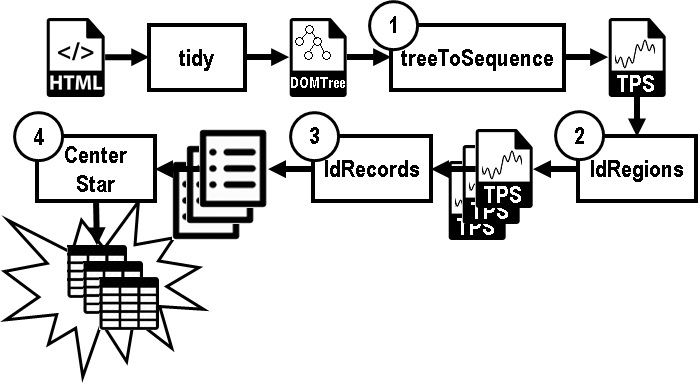
\includegraphics[width=208pt]{img/proposal.jpg}
  \caption{Extraction system overall diagram.}
  \label{fig:overall}
\end{figure}
%\vspace{0.67cm}

\subsection{Sequence Representation}\label{ss:seq}
Most of the works in this area use the DOM tree to represent the documents
subjected to record extraction. We choose, instead, an alternative
representation: a sequence of tag paths. This representation allows us to see
the web page as a sequence instead of a tree, enabling us to make use of
algorithms targeted at sequences. Such a representation was used before in
\cite{TPC09, SuffixTree12, TPS2013}.

The translation process from DOM tree representation to tag path sequence is
depicted in Figure \ref{fig:tree2seq}. The HTML code is converted to a DOM tree
in Step 1; the DOM tree is converted to a sequence of tag paths in Step 2 and;
in Step 3 the TPS is built by assigning TPCodes to each tag path. 

\begin{figure}[H]
  \centering
     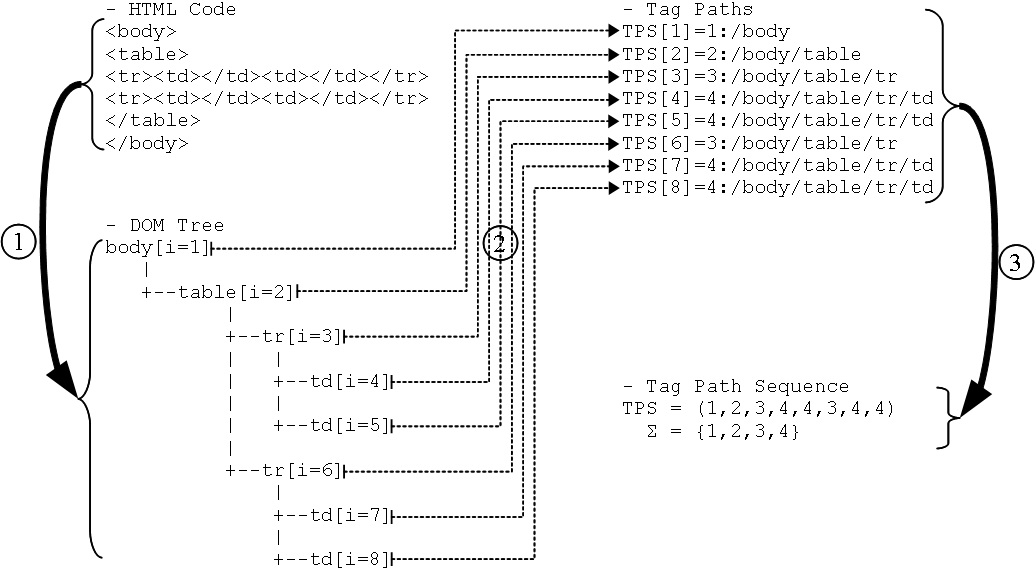
\includegraphics[width=\columnwidth]{img/tree2seq.jpg}
  \caption{tag path sequence built from HTML code snippet.}
  \label{fig:tree2seq}
\end{figure}

Algorithm \ref{alg:tree2seq} presents the TPS build process.
It is basically a depth first search that assembles the path from the root of
the tree to every other node and assigns a code to each distinct path found. To
help distinguish different regions of the document, during the region
identification step, we've added style definitions to the tag paths, similar to
what was done in \cite{grigalis2013towards} with the difference that here we use class
and in-line style attributes instead of rendering the entire document, avoiding
the computational cost associated with such a task.

\begin{algorithm}[h]
\caption{Builds a tag path sequence from a DOM tree}
\label{alg:tree2seq}
\begin{algorithmic}[1]
\Procedure{treeToSequence}{node,tp,tps by ref.}
\State $tp \leftarrow
concat(tp,$``/''$,node.$tag$,node.style)$\label{lin:alg:tree2seq:a}
\If {$tp \ni tagPathMap$} \label{lin:alg:tree2seq:b}
\State $tagPathMap \leftarrow tagPathMap \cup \{tp\}$ 
\State $tagPathMap[tp].code \leftarrow tagPathMap.size$ 
\EndIf \label{lin:alg:tree2seq:c}
\State $tps \leftarrow
concat(tps,tagPathMap[tp].code);$\label{lin:alg:tree2seq:d}
\For {each $child$ of $node$}
\State $treeToSequence(child,tp,tps)$\label{lin:alg:tree2seq:e} 
\EndFor 
\EndProcedure
\end{algorithmic}
\end{algorithm}

\textbf{Description of Algorithm \ref{alg:tree2seq}:} procedure
\texttt{treeToSequence} is initially called with the tree's root node, an empty
tag path string and an empty sequence: \\\texttt{treeToSequence}\texttt{(root,
``'', tps = ``'')}. In Line \ref{lin:alg:tree2seq:a} the current tag path string is
assembled; in Lines \ref{lin:alg:tree2seq:b}--\ref{lin:alg:tree2seq:c} the tag
path code is retrieved, if it is a recurring path, otherwise a new, ascending,
code is assigned to it and the path string is stored for future reference; In
Line \ref{lin:alg:tree2seq:d} the current TPCode is appended to the TPS and; In
Line \ref{lin:alg:tree2seq:e} the procedure is called recursively for every
child of the current node. When the procedure returns, the full TPS is stored in
parameter \texttt{tps} which was passed by reference.

\subsection{Region Identification}\label{ss:regi}

Before extracting the records themselves we first isolate the regions that
contain structured data. It is simpler and easier to extract records from a
delimited region that is known to contain structured data than it is to do so
from the entire document. The reason for this is that structured regions are
cyclic, i.e., since the records have similar structure and are contiguous then
its tag path sequence will display a cyclic behaviour as illustrated in Figure
\ref{fig:stru}.

We can see in Figure \ref{fig:stru} that whenever there is structured
content in the document (i.e., repeating records with similar structure), be it
the main content, menus, or anything else, the corresponding interval in the
sequence displays a cyclic behaviour (the encircled subsequences in Figure
\ref{fig:stru}).
In other words, the sequence stabilizes during the structured portions. That
happens because the records look alike and so their paths and styles repeat
themselves. We took advantage of this observation to devise Algorithm
\ref{alg:idreg} that isolates the structured segments of the sequence.

\begin{algorithm}
\caption{Identifies structured regions in a document}
\label{alg:idreg}
\textbf{Input:} tag path sequence \\
\textbf{Output:} a set of structured regions

\begin{algorithmic}[1]

\Function{IdRegions}{tps} \Comment{Main Function}
\State $tpsContour \leftarrow \Call{contour}{tps}$
\State $regions \leftarrow \Call{segment}{tpsContour}$
\State $regions \leftarrow \Call{mergeRegions}{regions}$
\State $regions \leftarrow \Call{filterRegions}{regions}$
\State \Return $regions$
\EndFunction

%\\\hrulefill

\Function{contour}{tps} \Comment{Subroutine}\label{line:alg:idreg:contour:begin}
\State $maxHeight \leftarrow 0$ 
\For {$i \leftarrow 1..length(tps)$}\label{line:alg:idreg:a}
\If {$tps[i]>maxHeight$}\label{line:alg:idreg:b}
\State $maxHeight \leftarrow tps[i]$ 
\EndIf 
\State $contour[i] \leftarrow maxHeight$ 
\EndFor\label{line:alg:idreg:c} 
\State \Return $contour$ \label{line:alg:idreg:d} 
\EndFunction\label{line:alg:idreg:contour:end}

%\\\hrulefill

\Function{segment}{contour} \Comment{Subroutine}
\State $diff \leftarrow difference(contour)$\label{line:alg:idreg:e}
%\State $diff \leftarrow concat(diff, 1)$
\State $regions \leftarrow \emptyset$\label{line:alg:idreg:f}
\State $start \leftarrow 1$
\State $end \leftarrow 1$
\For{$i \leftarrow 1..length(diff)$}
\If {$diff[i] \neq 0$}
\If {$start \neq end$}
\State $regions \leftarrow regions \cup [start, end)$
\EndIf
\State $start \leftarrow i + 1$
\State $end \leftarrow i + 1$
\Else
\State $end \leftarrow end + 1$
\EndIf
\EndFor\label{line:alg:idreg:g}
\State \Return $regions$\label{line:alg:idreg:h}
\EndFunction

%\\\hrulefill

\Function{mergeRegions}{regions} \Comment{Subroutine}
\State $merged[1] \leftarrow regions[1]$
\State $j \leftarrow 1$ 
\For {$i \leftarrow 2..regions.count()$}\label{line:alg:idreg:i}
\State $\Sigma_{prev} \leftarrow alphabet(merged[j])$ \label{line:alg:idreg:j}
\State $\Sigma_{curr} \leftarrow alphabet(regions[i])$
\If {$\Sigma_{prev}\cap\Sigma_{curr} \neq \emptyset$}
\State $merged[j] \leftarrow concat(merged[j], regions[i])$
\Else 
\State $j \leftarrow j + 1$ 
\State $merged[j] \leftarrow regions[i]$ 
\EndIf \label{line:alg:idreg:k}
\EndFor
\State 
\Return $merged$ \label{line:alg:idreg:l}
\EndFunction

%\\\hrulefill

\Function{filterRegions}{regions} \Comment{Subroutine}
\For{each region in regions}\label{line:alg:idreg:m}
\State $angCoef \leftarrow linearRegression(region)$\label{line:alg:idreg:n}
\If{$|angCoef| > threshold$}\label{line:alg:idreg:o}
\State $regions \leftarrow regions - \{region\}$\label{line:alg:idreg:p}
\EndIf
\EndFor
\State \Return $regions$\label{line:alg:idreg:q}
\EndFunction

\end{algorithmic}
\end{algorithm}

\textbf{Description of \texttt{idRegions} function:} this is the main function
that calls the other subroutines. It receives a TPS as input and returns the
detected structured regions as output;

\textbf{Description of \texttt{contour} function:} this function is
pretty straightforward, it receives the TPS as input, iterates over the sequence (Line
\ref{line:alg:idreg:a}), computes its upper contour (i.e., the maximum value
seen so far) in Lines \ref{line:alg:idreg:b}--\ref{line:alg:idreg:c} and then;
returns the sequence's contour (Line \ref{line:alg:idreg:d});

\textbf{Description of \texttt{segment} function:} this function receives the
sequence's contour as input, computes its finite difference (Line
\ref{line:alg:idreg:e}), as defined in Definition \ref{def:diff};
assembles a set with all intervals where the finite difference is zero-valued
(Lines \ref{line:alg:idreg:f}--\ref{line:alg:idreg:g}) and then; returns this
set of possibly structured regions (Line \ref{line:alg:idreg:h});

\textbf{Description of \texttt{mergeRegions} function:} this function
receives, as input, a set of possibly structured regions; iterates over this set (Line
\ref{line:alg:idreg:i}), merging the adjacent elements with intersecting alphabets (Lines
\ref{line:alg:idreg:j}--\ref{line:alg:idreg:k}) and then; returns the merged set
of possibly structured regions (Line \ref{line:alg:idreg:l});

\textbf{Description of \texttt{filterRegions} function:} this function
receives, as input, a set of possibly structured regions; iterates over this set (Line
\ref{line:alg:idreg:m}); computes the linear regression for each region in the
set (Line \ref{line:alg:idreg:n}); if the current region has an angular
coefficient above the threshold (Line \ref{line:alg:idreg:o}) it is removed from the set
(Line \ref{line:alg:idreg:p}) and finally; the remaining set of regions is
returned (Line \ref{line:alg:idreg:q}).

\begin{figure*}[h]
 %\captionsetup{width=\textwidth}
  \centering
     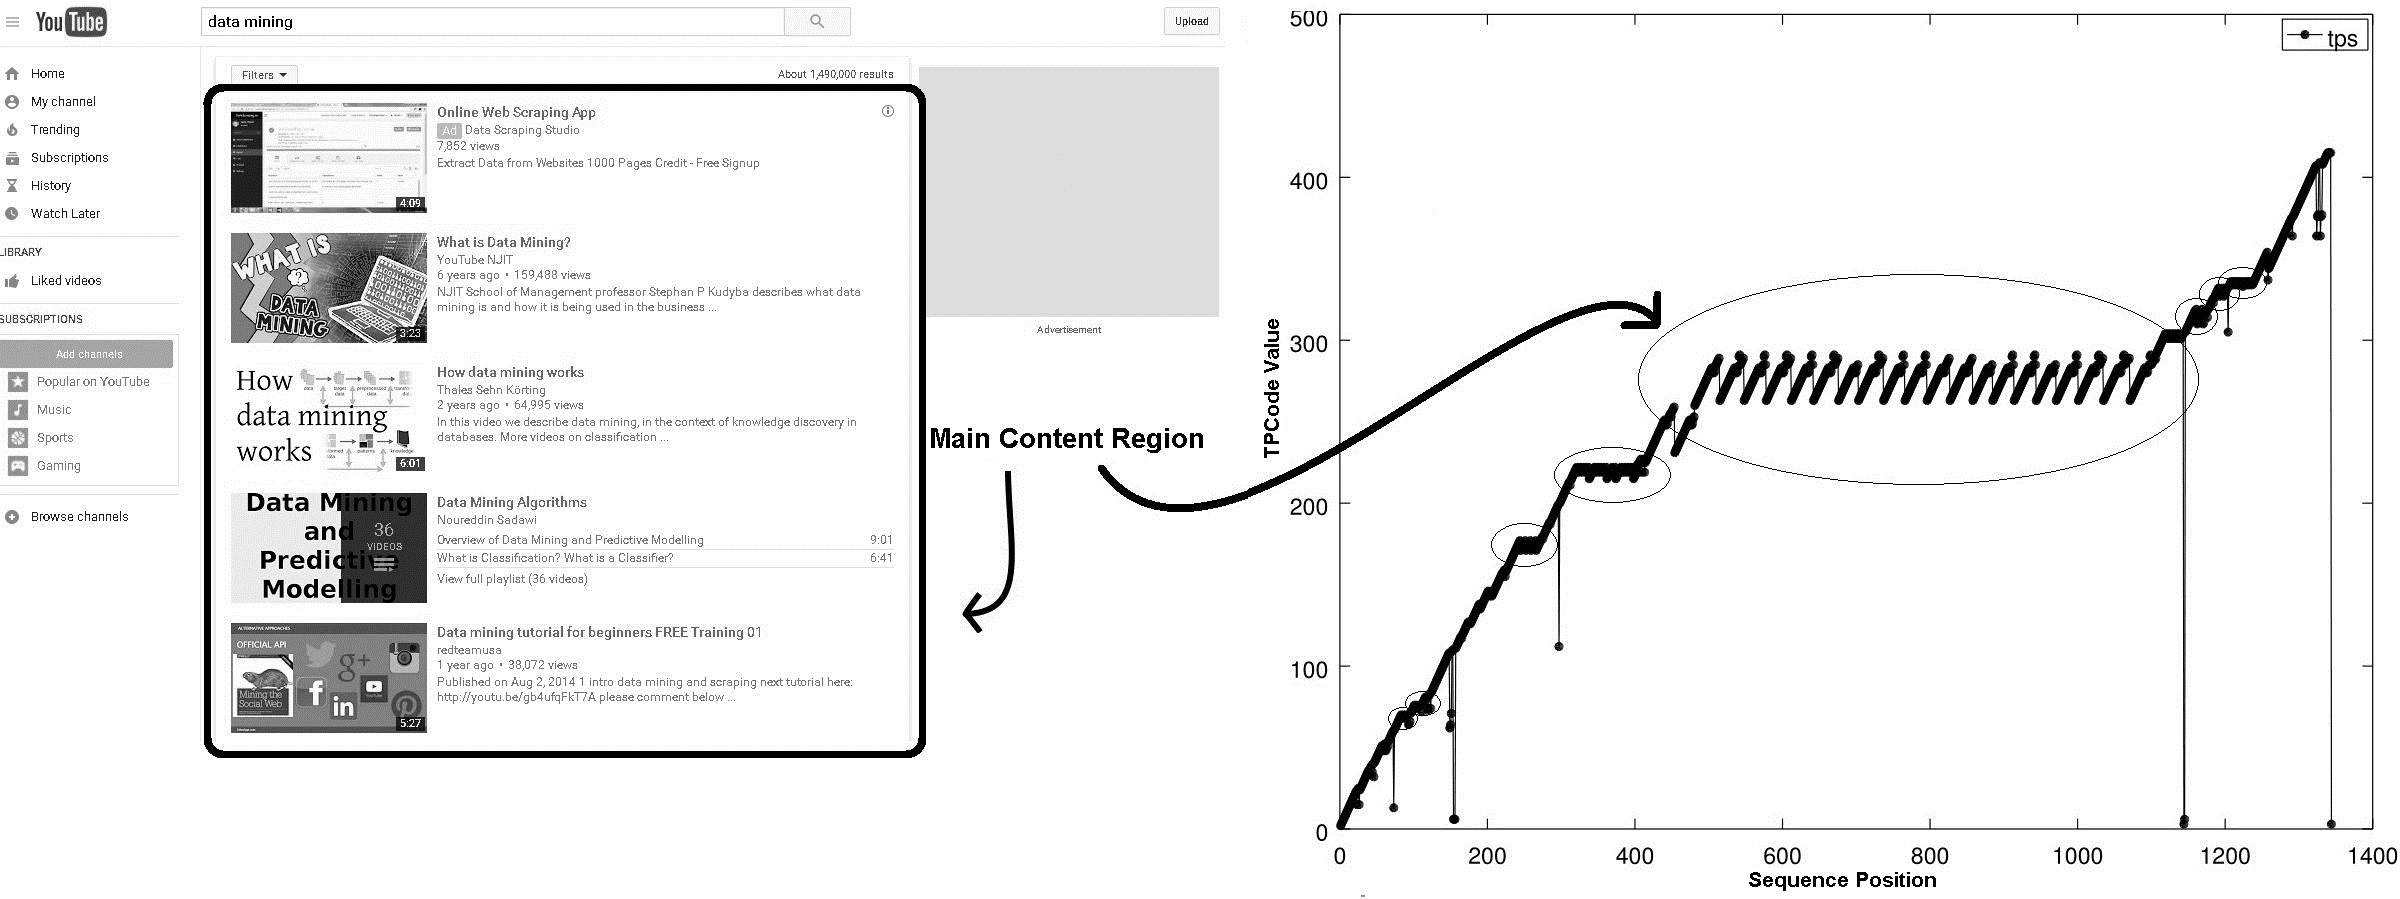
\includegraphics[width=\textwidth]{img/main-reg.jpg}
  \caption{How structured content appears in the sequence (structured regions encircled).}
  \label{fig:stru}
\end{figure*}

Algorithm \ref{alg:idreg} starts by computing the contour of the input sequence,
in function \texttt{contour}, and its finite difference, in function
\texttt{segment}, using this to segment the document into several regions.
The idea behind function \texttt{segment} is that the finite difference of
the contour will be zero whenever the contour stabilizes (i.e., when it
remains constant during an interval). As we can see in Figure
\ref{fig:contour}a there are flat (constant) intervals in the sequence's
contour and consequently the first difference will be zero during those
intervals, as shown in Figure \ref{fig:contour}b.

\begin{figure}[h]
  \centering
     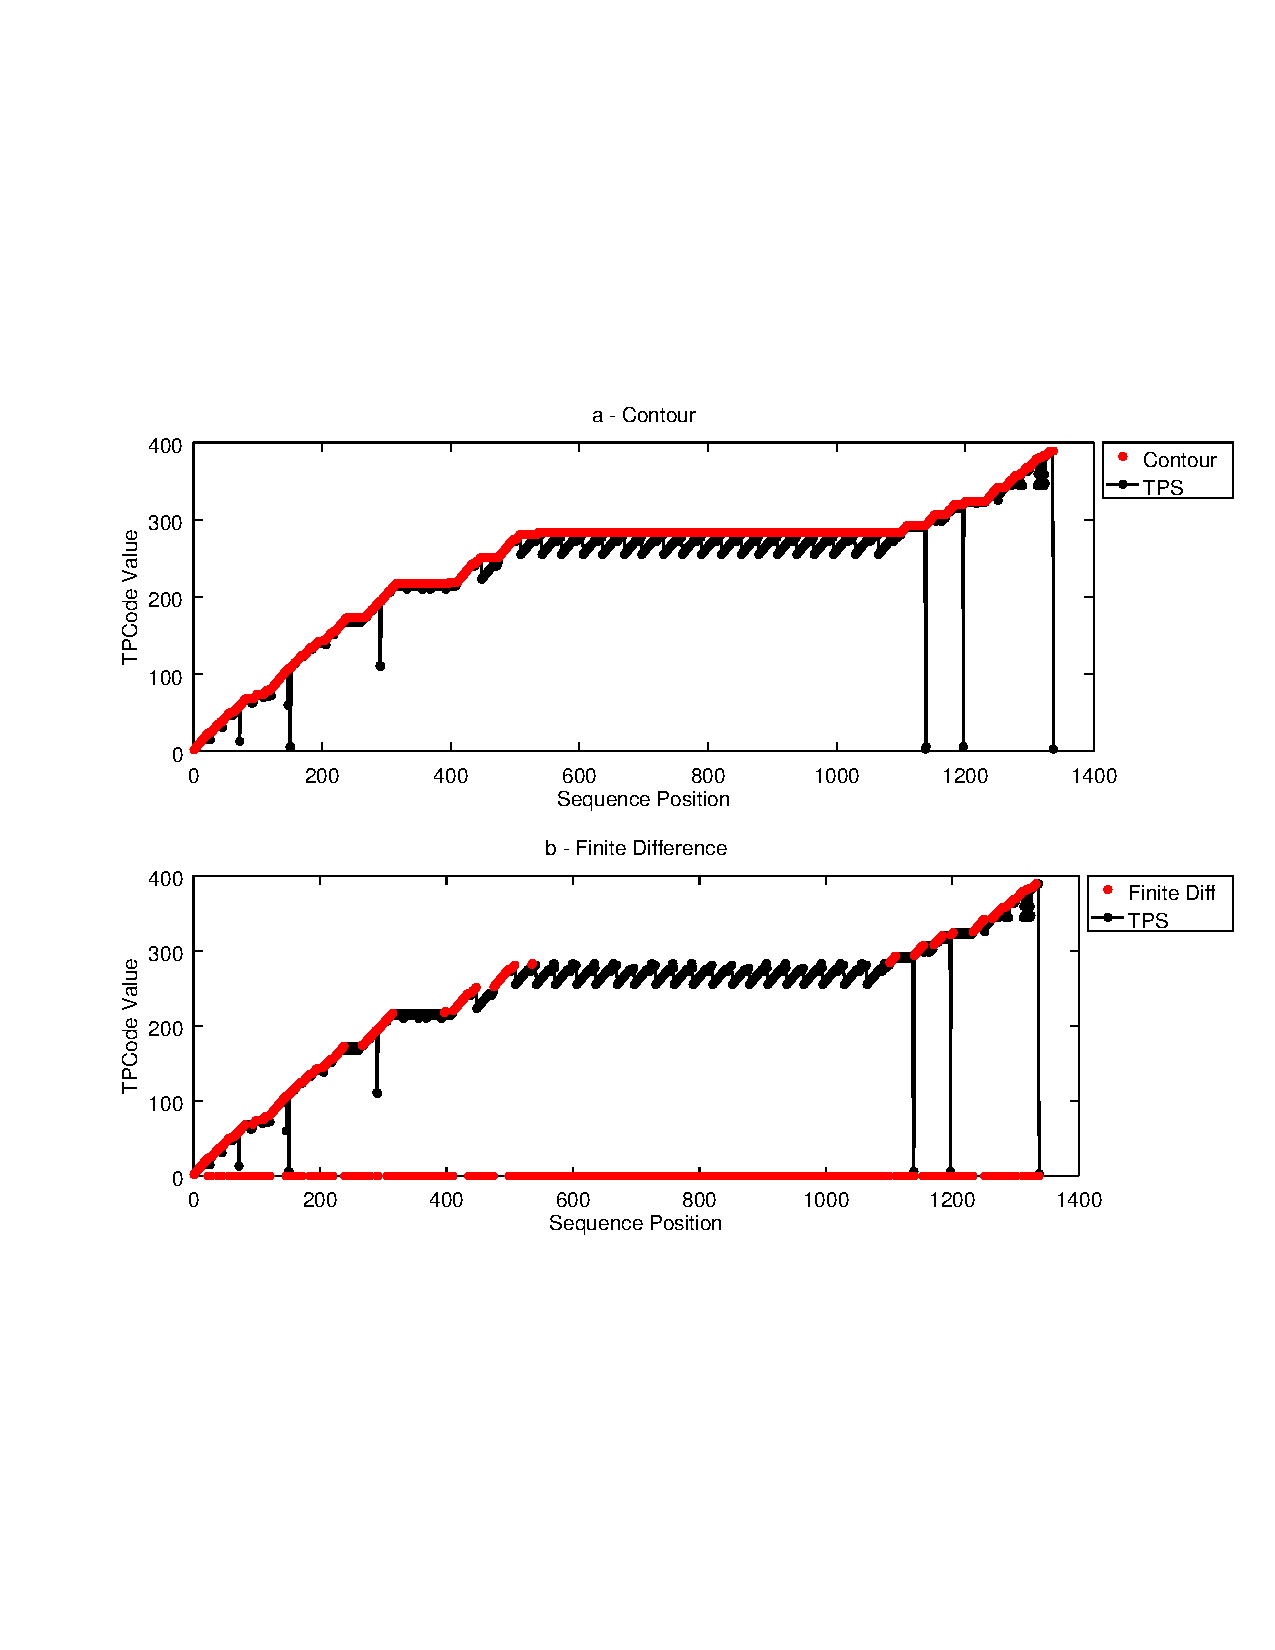
\includegraphics[trim={2.5cm 7.5cm 1cm 6.5cm}, width=\linewidth
     ]{img/contour.pdf}
  \caption{a) Contour of a TPS; b) Finite difference of contour.}
  \label{fig:contour}
\end{figure}

The resulting regions are then merged together according to their alphabets
(i.e., set of symbols that form the sequence). If two adjacent regions share a
common alphabet, they are merged into a single region, if their alphabet is
disjoint (i.e., they share no common symbols) they are kept apart.

At last, to ensure that the identified regions contain structured content, they
are filtered out according to their angular coefficient. This filtering step is
necessary because when using the contour and its difference to segment the
sequence, it is possible that some of the identified regions are spurious. If a
region is indeed cyclic, its linear regression will yield a small angular
coefficient. If it is not cyclic, then it is either increasing or decreasing and
in both cases the linear regression will yield a much greater angular
coefficient.

The computational complexity of functions $contour$ and $segment$ are linear in
the size of the input sequence. For functions $mergeRegions$ and $filterRegions$
the complexity is linear in the number of regions detected, which in turn have a
worst case proportional to the size of the sequence, so the overall time
complexity for function $idRegions$, in the worst case, is $O(n)$ where $n$ is
the size of the sequence.

After processing the regions with function \texttt{idRegions} there is an
optional, and application dependent, step: deciding which regions are content
and which are noise. Here we chose to identify the main content and rule out
menus and advertising. The approach we've adopted for this task consists of
assigning a score to each region and separate them into two clusters, using an
optimal 1D k-means algorithm\cite{1dkmeans2011}. The cluster with lower centroid
is discarded and the remaining cluster is kept as content. The algorithm in
\cite{1dkmeans2011}, although it runs in $O(n^2)$ time, in practice it doesn't
have a significant impact on run time because it is proportional to the number
of regions and not to the size of the document (though, in worst case, the
number of regions could escalate to a value proportional to the document size,
this is not the average behaviour displayed in Figure \ref{fig:runtime}).

The score of a region is computed as defined in Equation \ref{eq:scorereg},
where \texttt{positionScore} means the distance of the region to the center of
the sequence (the lower the score, the greater the distance of the region from
the center of the sequence) and \texttt{sizeScore} means the percentage of the
sequence occupied by the region. Both \texttt{positionScore} and
\texttt{sizeScore} vary from 0.00 to 1.00. \texttt{maxDistance} is equal to
$\frac{tpsSize}{2}$ because that is the maximum distance a region can be from
the center of the TPS. The final \texttt{score} is the arithmetic mean of both
scores. The higher the region's score the more likely it represents content
rather than noise.

\begin{equation}\label{eq:scorereg}
\begin{split}
positionScore \leftarrow 1-\frac{|tpsCenter - regionCenter|}{maxDistance}, \\
sizeScore \leftarrow \frac{length(region)}{tpsSize},\\
score \leftarrow \frac{positionScore+sizeScore}{2}
\end{split}
\end{equation}

\subsection{Record Identification}\label{ss:reci}

For each region identified in the previous step we now try to extract records
out of it. To do so, we analyse the tag paths that appear in the sequence
against the region's spectrum (Definition \ref{def:dft}). The spectrum is
calculated using the FFT\cite{fft1965} (Definition \ref{def:fft}).
The FFT factors the sequence into its frequency components, so
cyclic sequences will exhibit higher peaks in frequencies that correspond to the
main period of the sequence as we can see in Figure \ref{fig:fftreg} (the main
content region of Figure \ref{fig:stru}). Figure \ref{fig:fftreg}a shows the
subsequence that represents a structured region of the TPS and, hence, displays
a cyclic behaviour and a linear regression with a small angle. In this case the
linear regression displays an inclination of only 0.15 degrees (almost
horizontally flat), if the region were unstructured (i.e., an increasing or
decreasing subsequence) its angular coefficient would be much higher (e.g., 45
degrees of inclination); Figure \ref{fig:fftreg}b shows the subsequence's PSD
with a highlighted frequency peak. The frequency peak is located at position 20
of the spectrum, which corresponds exactly to the number of records present in
this region and if we divide the size of the region by the number of records we
get the average record size (approximately 31 in this case).
In short, this frequency peak represents the record count (or number of cycles
in the subsequence) and its corresponding period (i.e., the subsequence length
divided by the frequency) is equivalent to the average record size.

\begin{figure}[h]
  \centering
     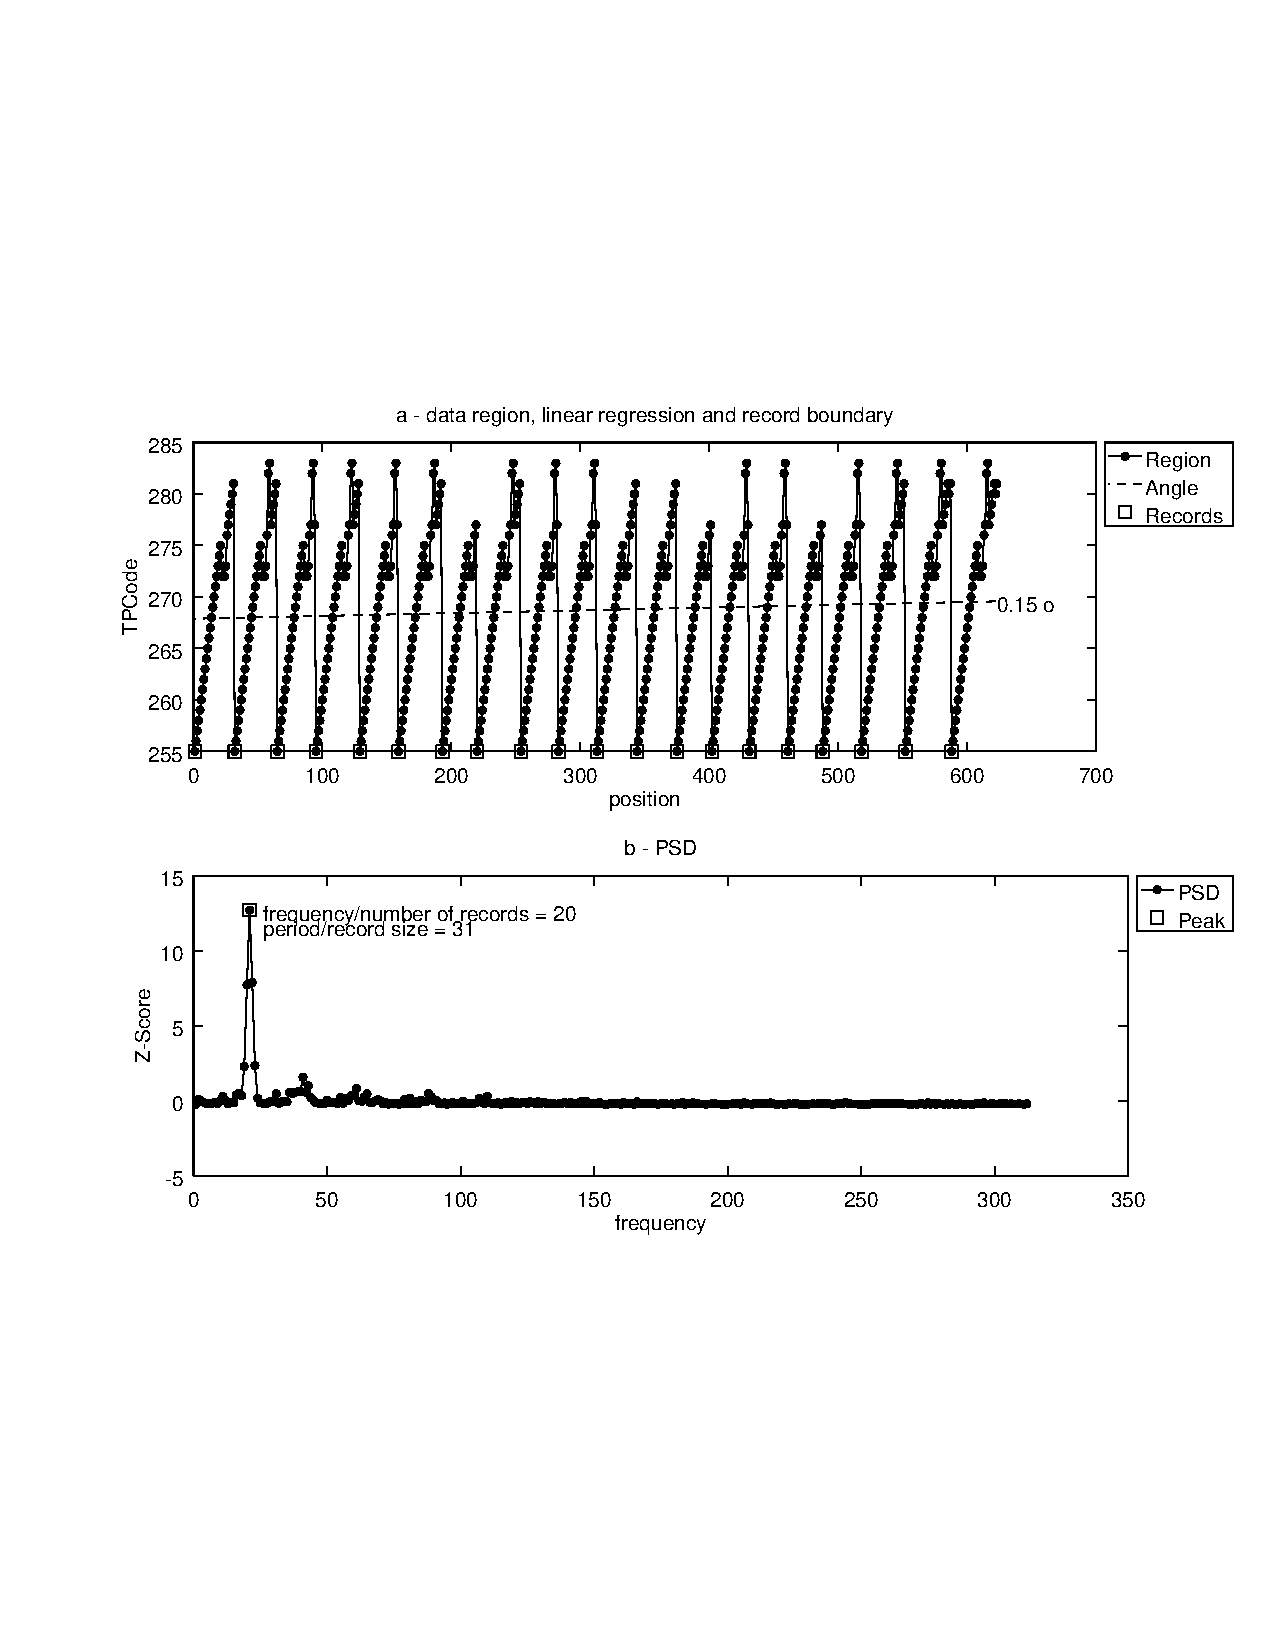
\includegraphics[trim={2.5cm 7.5cm 1cm 6.5cm}, width=\linewidth
     ]{img/fftreg.pdf}
  \caption{a) The cyclic behaviour of a structured region; b) The PSD of a
  structured region.}
  \label{fig:fftreg}
\end{figure}

To decide if a certain TPCode represents a record boundary within the region, we
check how well distributed along the subsequence each TPCode is, in increasing
order, using the coefficient of variation (CV for short -- Definition
\ref{def:cv}) of the distance between its occurrences, e.g., if a given tag path
occurs at positions \{10, 20, 30\}, the distances between consecutive
occurrences are \{$20-10 = \textbf{10}$, $30-20 = \textbf{10}$\} and the CV is
equal to 0.0\% since all distances are the same. In order to determine if a tag
path is well distributed a threshold must be set. Since the regions are cyclic,
the number of different tag paths that form the region's sequence is much
smaller when compared to the size of the sequence. This is due to inherent
repetitions and so it is not prohibitive to check the CV of every symbol in the
region's alphabet. Figure \ref{fig:fftreg}a exhibits the record boundaries
detected for that region (highlighted with squares). In this case the TPCode with
value 255 matches the spectrum and CV constraints as we shall see. TPCode 255
occurs 20 times at positions \{1, 32, 65, 95, 129, 159, 193, 220, 254, 283, 313,
344, 375, 402, 431, 461, 488 518, 552, 588\} and the distance between adjacent
occurrences are \{31, 33, 30, 34, 30, 34, 27, 34, 29, 30, 31, 31, 27, 29, 30,
27, 30, 34, 36\} so the average record size, for this TPCode, is 30.895, the
standard deviation is 2.6435 and the CV is equal to 0.085564. If we validate
this information against the region's spectrum we'll have a match because both
the number of occurrences (frequency) and the average size (period) match the
peak encountered in the region's spectrum at position 20 and the CV for this
TPCode is only about 8.5564\% (a low CV means little variation in record size).

Cross validating TPCode variation against the TPS spectrum is more robust than
doing the inverse (i.e., selecting the highest peak in the spectrum and then
searching for a corresponding TPCode). This is because the signal may be noisy
and the spectrum may contain artifacts and errors due to windowing (e.g.,
spectral leakage) and frequency resolution limitation, and so it is not
guaranteed that the highest peak will in fact correspond to the correct
period.
Figure \ref{fig:fftleak} shows an example of this situation where the highest
peak in the spectrum is not the correct period, but nonetheless there is a
significant peak that corresponds to the correct period. Figure
\ref{fig:fftleak}a shows a structured region with a cyclic behaviour, much like
Figure \ref{fig:fftreg}a, except that, this time, the highest frequency peak
in Figure \ref{fig:fftleak}b does not correspond to the correct period, but
still, there is a significant frequency peak that matches the correct period
and record count.


\begin{figure}[h]
  \centering
     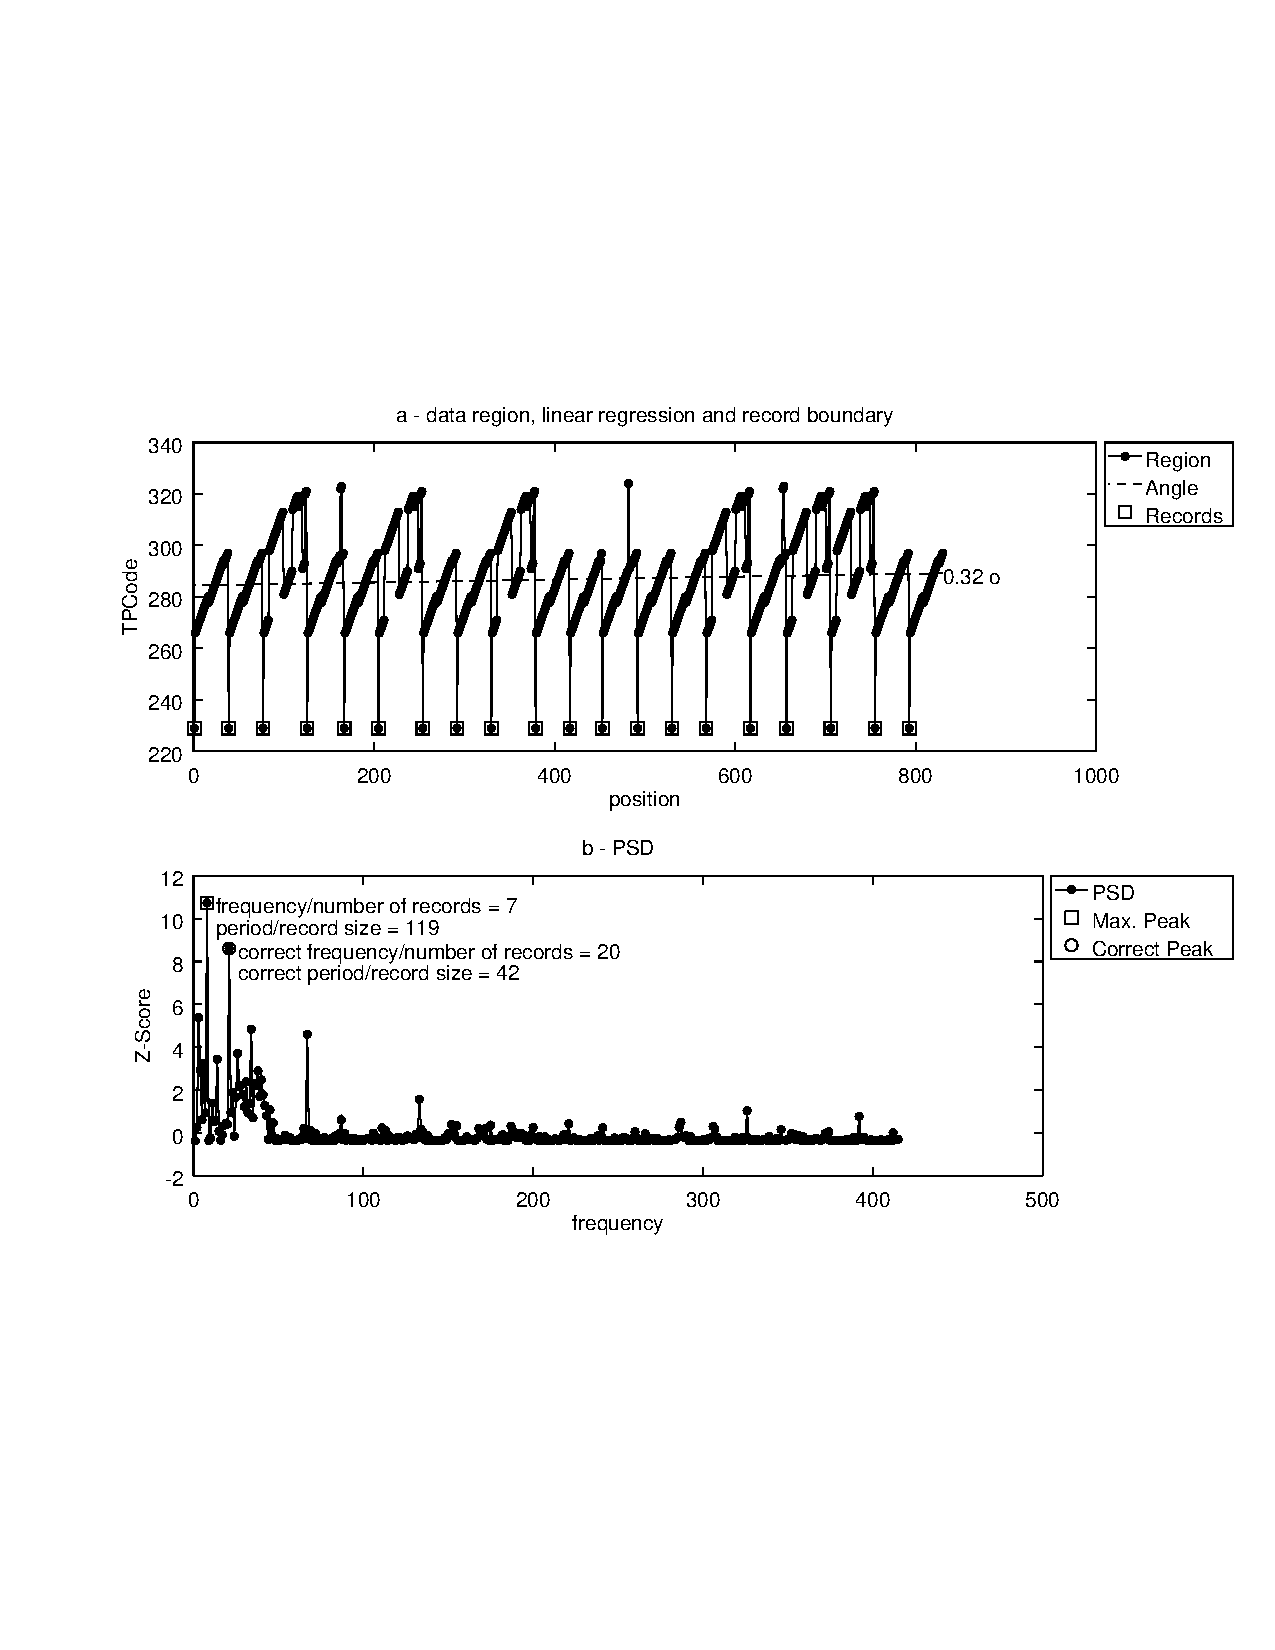
\includegraphics[trim={2.5cm 7.5cm 1cm 6.5cm}, width=\linewidth
     ]{img/fftleak.pdf}
  \caption{An example when the maximum peak in the spectrum does not correspond to the correct period.}
  \label{fig:fftleak}
\end{figure}

For those tag paths that are well distributed along the sequence, we search the
corresponding range of the spectrum for a significant peak. If such a peak is
found we subdivide the region accordingly, extract the records and end the
process. To determine if a peak is significant we convert the spectrum to
\textit{z-score} (Definition \ref{def:zscore}) and set a threshold measured in
number of standard deviations.

Algorithm \ref{alg:idrec} along with Figure \ref{fig:fftreg} shows in more
detail the process of identifying the records within a region.

\begin{algorithm}
\caption{Locates record boundaries in a region}
\label{alg:idrec}
\textbf{Input:} a region's TPS \\
\textbf{Output:} a set of record starting positions

\begin{algorithmic}[1]

\Function{IdRecords}{region}
\State $signal \leftarrow region-\mu(region)$ \Comment{remove DC}
\State $PSD \leftarrow abs(FFT(signal))^2$\label{line:alg:idreg:r}
\State $\Sigma \leftarrow sort(alphabet(region), ascending)$
\For{each $symbol$ in $\Sigma$}\label{line:alg:idreg:s}
\State $recordPositions \leftarrow find(region == symbol)$
\State $recSize \leftarrow difference(recordPositions)$
\State $recCount \leftarrow length(recordPositions)$
\State $CV \leftarrow
\frac{\sigma(recSize)}{\mu(recSize)}$\label{line:alg:idreg:t}
\If{$CV < CVthreshold$}\label{line:alg:idreg:u}
\State $interval \leftarrow [recCount-2 .. recCount+2]$
\If{$PSD[interval] > numSD \cdot \sigma(PSD)$}\label{line:alg:idreg:v}
\State \Return $recordPositions$\label{line:alg:idreg:w}
\EndIf
\EndIf
\EndFor
\State \Return $\emptyset$
\EndFunction

\end{algorithmic}
\end{algorithm}

\textbf{Description of Algorithm \ref{alg:idrec}:} function \texttt{IdRecords}
receives, as input, a structured region; it computes the PSD (Definition
\ref{def:dft}, Equation \ref{eq:psd}) of the input sequence using the FFT
(Definition \ref{def:fft} -- Line \ref{line:alg:idreg:r}); iterates over the
region's alphabet, in ascending order (Line \ref{line:alg:idreg:s}); for each
symbol in the alphabet its CV is calculated (Line \ref{line:alg:idreg:t}), as
defined in Definition \ref{def:cv}, and checked against a threshold (Line
\ref{line:alg:idreg:u}); if it is bellow the threshold (meaning the current
symbol is well distributed along the sequence) then the PSD is scanned in the
range around the number of candidate records (Line \ref{line:alg:idreg:v} --
\texttt{recCount} is the frequency we are validating against the sequence's
spectrum) and; if a considerable peak is found in this range the function
returns the positions of the current symbol (Line \ref{line:alg:idreg:w}).

With respect to \texttt{idRecords}' time complexity, the overall complexity is
dominated by Line \ref{line:alg:idreg:r}, which is $O(nlogn)$ on the size of the
input region.
\subsection{Record Alignment}\label{ss:reca}

Once the records are identified they need to be correctly aligned (i.e., their
fields must the matched in the best possible way) so they can be extracted in
tabular form.

The problem of optimal multiple sequence alignment is known to be
NP-Hard\cite{msanphard2006}, so we are forced to adopt approximate solutions for
this problem, one such solution, known as \textit{Center
Star}\cite{centerstar1993}, has a polynomial time complexity and guaranteed
error bound. This algorithm uses the edit distance to align two sequences and
works by inserting ``spaces'' in the sequences when a misalignment is found. It
also makes no assumptions about the data being aligned (i.e., it is general)
and runs in time proportional to $O(k^2n^2)$, where $k$ is the number of records to be
aligned and $n$ is the size of the records. The multiple alignment score (i.e.,
the sum of pairs edit distance) for the approximate solution is guaranteed to be
at most a factor of 2 worst than the optimal solution's score and in practice
can be better than this for similar strings, according to \cite{centerstar1993}.

Table \ref{table:align} shows the resulting alignment, using \textit{Center
Star} method, for the records extracted from the region depicted in Figure
\ref{fig:fftreg}a. The values in the cells are
TPCodes, so each represents a distinct node in the DOM tree and the empty
cells are the spaces introduced by \textit{Center Star} algorithm
during sequence alignment.

The alignment of records, by itself, deserves a more in depth study. It is still
an open, and very important, problem related to web record extraction. As
observed in \cite{listExtract2009}, there is no single correct answer when it
comes to the alignment of records and this constitutes an additional difficulty
when evaluating the correctness of an alignment.

\begin{table}[h]
\centering
\caption{\textit{Center Star} -- result of record alignment for region in Figure
\ref{fig:fftreg}a.}
\label{table:align}
\begin{tiny}
\setlength\tabcolsep{2.3pt}
\begin{tabular}
{|c|l|l|l|l|l|l|l|l|l|l|l|l|l|l|l|} \hline
rec \#&\multicolumn{15}{c|}{fields (TPCodes)}\\ \hline
 \#1&255&256&258&259&262&266&270&272&270&270&274&   &   &   &278\\ \hline
 \#2&255&256&258&259&262&266&270&272&270&270&   &280&   &274&278\\ \hline
 \#3&255&256&258&259&262&266&270&272&270&270&274&280&274&   &   \\ \hline
 \#4&255&256&258&259&262&266&270&272&270&270&274&280&   &274&278\\ \hline
 \#5&255&256&258&259&262&266&270&272&270&270&274&280&   &274&   \\ \hline
 \#6&255&256&258&259&262&266&270&272&270&270&274&280&   &274&278\\ \hline
 \#7&255&256&258&259&262&266&270&272&270&270&274&   &   &   &   \\ \hline
 \#8&255&256&258&259&262&266&270&272&270&270&274&280&   &274&278\\ \hline
 \#9&255&256&258&259&262&266&270&272&270&270&   &280&   &274&   \\ \hline
\#10&255&256&258&259&262&266&270&272&270&270&274&280&   &274&   \\ \hline
\#11&255&256&258&259&262&266&270&272&270&270&274&   &   &   &278\\ \hline
\#12&255&256&258&259&262&266&270&272&270&270&274&   &   &   &278\\ \hline
\#13&255&256&258&259&262&266&270&272&270&270&274&   &   &   &   \\ \hline
\#14&255&256&258&259&262&266&270&272&270&270&   &280&   &274&   \\ \hline
\#15&255&256&258&259&262&266&270&272&270&270&274&280&   &274&   \\ \hline
\#16&255&256&258&259&262&266&270&272&270&270&274&   &   &   &   \\ \hline
\#17&255&256&258&259&262&266&270&272&270&270&274&280&   &274&   \\ \hline
\#18&255&256&258&259&262&266&270&272&270&270&274&280&   &274&278\\ \hline
\#19&255&256&258&259&262&266&270&272&270&270&274&280&274&278&278\\ \hline
\#20&255&256&258&259&262&266&270&272&270&270&274&280&274&   &   \\ \hline
\end{tabular}
\end{tiny}%}
\end{table}

It is important to note that the previous step of record identification
is parametrized by the CV of record size and this parameter directly affects the
quality of the alignment in the following way: the lower the CV the better will
be the alignment at the expense of recall, i.e., we can filter out records too
different in size because such records are more prone to misalignment and that
degrades the quality of the extraction. As stated in \cite{centerstar1993}, 
similar sequences yield better alignment results. The structure of the
records detected by our algorithm is necessarily similar, otherwise the
data region would not be cyclic, but the size of the records can vary as a
consequence of optional and disjoint fields that may be present.
So, if we enforce a low CV we can also guarantee that the records will have
similar size improving overall record similarity.

Another measure we take, in order to improve alignment quality, is to prune the
records before aligning them. Since we are not constrained here by the hierarchy
imposed by the DOM's tree structure, we can remove intermediate nodes that do
not contain information, easing the alignment process and improving both it's
quality and running time (since the input size is diminished).

\section{Experiments}\label{sec:result}

In this section, we discuss and compare the results of our research with other
approaches found in the literature that we considered to be most relevant. The
proposals we considered most relevant are those which are fully automatic,
highly effective (i.e., high f-score), domain independent and computationally
efficient.

The main difficulty we encountered when trying to compare our results with the
results of the others, was the unavailability of implementations (despite
contacting the authors). For this reason we were unable to make a deeper and
independent comparative analysis.
Had implementations been available one could compare specific situations where
one approach performs better than the other, otherwise we can only compare
against published results (usually summarized precision and recall).
%Although several works have criticized this aspect, few provided implementations.

Furthermore, implementing approaches proposed by others is also a complex
matter. For starters, most papers do not provide full details (maybe due to
space constraints?) and there is no guarantee that an independent implementation
will match exactly the one used by the authors in their experiments.
% and that invalidates the effort.

We have implemented our approach using a two tier software architecture where
the core is coded in C++ and the presentation layer (graph plotting, result
manipulation / display, logging, timing, etc.) in embedded Lua \cite{luahome}.
For HTML parsing we've linked our system against libtidy\cite{libtidy}. Our
implementation is publicly available at
GitHub\footnote{\url{https://github.com/rpvelloso/webMining.git}} and we
encourage and support the scientific community to build on top of it, run
independent experiments, implement other techniques for the sake of comparison
and so on.
%Appendix \ref{app:a} has a simple usage example of our system and the
%infrastructure we have exposed to the Lua environment.
% (there is also an integrated relational database available to the user --
% SQLite\cite{sqlite}).

We used three datasets for comparison, two of them are commonly used for
benchmarking and the other one was compiled by ourselves with pages collected
from top largest internet companies\footnote{most pages were drawn from domains
owned by the companies listed here:
\url{https://en.wikipedia.org/wiki/List_of_largest_Internet_companies}.}
websites with more up to date templates from various domains (the documents were
collected in may/2017). Dataset $\#1$ was proposed by \cite{yamada2004testbed}
and consists of 5 pages per site and 51 sites randomly sampled out of 114,540
pages. This dataset was used, among others, by \cite{TPC09,grigalis2013towards}
which, in our opinion, are relevant works in the field, specially when we
consider the requirements of being unsupervised, efficient, effective and HTML
syntax independent. They are also relatively recent.
Dataset $\#2$ was assembled and used in \cite{grigalis2013towards} and consists
of 3 pages per site and 10 sites picked by the author. Dataset \#3 was assembled
by ourselves and consists of 46 sites from various domains, 1 page per site. To
better evaluate and demonstrate the effectiveness of our approach we needed more
recent and up to date site templates in our test cases, that is the reason we
added this third dataset to the experiments.
Table \ref{table:dataset} presents summarized information about the datasets.

\begin{table}[h]
\centering
\caption{Summarized dataset information.}
\label{table:dataset}
\begin{tabular}
{|l| c| c| c|}\hline
Dataset	& \#1	& \#2 & \#3 \\ \hline
Sites &	51 & 10 & 46\\ \hline
Pages per site	& 5 & 3 & 1\\ \hline
Average records & 21 & 22 & 32 \\ \hline
Total records &	1052 & 218 & 1466 \\ \hline
\end{tabular}
%}
\end{table}

The following parameters were used in the experiments: CV threshold $0.35$,
Z-Score threshold $9.5$ and angular coefficient threshold $4.5$ degrees. These
parameters were chosen empirically.

Table \ref{table:compare1} compares precision, recall and f-score of our
approach with three other state-of-the-art techniques, using dataset $\#1$:
MDR\cite{MDR03}, TPC\cite{TPC09} and ClustVX\cite{grigalis2013towards}.
Our approach performs better than MDR and TPC and slightly worse than ClustVX,
but on the other hand our technique doesn't need to render the entire page in
order to extract the records. As a matter of fact, we just parse the HTML and
don't even process CSS definitions (our approach just cares about \texttt{class}
attributes).
We've considered MDR to be of relevance here because it is one of the few
approaches with available implementation and probably the first to achieve
acceptable results (both in computational complexity and effectiveness).
The experimental results were manually inspected, one by one, to check if the
final alignment was acceptable (we say ``acceptable'' because there can be more
than one correct alignment), we have not yet devised metrics to automatically
measure the record alignment.

Table \ref{table:compare2} compares only against ClustVX, using dataset $\#2$.
Again we've performed slightly worse, but close to a perfect result. This
dataset is more up to date than dataset $\#1$, with respect to document
template and web programming practices.
% but it contains only a small number of
% documents so it is not an extensive, large scale, comparison.

Table \ref{table:compare3} presents the results obtained over our own dataset,
assembled with documents from large internet companies' websites using modern
and up to date layouts (since the documents were collected recently - may/2017)
from various distinct domains, including: travel (e.g., booking.com,
tripadvisor.com), real estate (e.g., airbnb.com), car rental and sales (e.g.,
rentalcars.com), search engines (e.g., google.com, yahoo.com), videos (e.g.,
youtube.com), movies (e.g., imdb.com), music (e.g., itunes.com), retail sales
(e.g., aliexpress.com, walmart.com, amazon.com) and social networks (e.g.,
facebook.com, linkedin.com). Despite a somewhat lower recall, 89.77\%, the
overall quality is still pretty good, 94.13\% f-score, due to the high (near
perfect) precision of 98.95\%. This high precision is a key factor when dealing
with web scale data and it is quite an achievement when we consider data
diversity and the fact that our approach is both automatic and computationally
efficient, such attributes are necessary for feasibility.

We have mentioned that an important requirement when dealing with web scale is
efficiency. On that subject ClustVX fails to deliver for two reasons: (1) it
employs a browser engine to render the entire web page and issues several calls
to the browser API during extraction and; (2) it clusters DOM tree nodes with
similar ``Xstrings'' (a variation of a tag path) probably using edit distance
(the paper is not clear about this issue) which has quadratic time complexity.
Anyway, we chose to compare against this approach mostly because the reported
results are near perfect and we wanted to show that our proposal achieves very
similar results without incurring in unnecessary computational cost. To support
our claim about the computational cost involved in document rendering, we have
compared running time of our approach using an internal HTML parser versus a
browser engine. The browser engine is controlled via
WebDriver\footnote{\url{https://www.w3.org/TR/webdriver/}} interface in offline
mode (to avoid computing networking latency as runtime).

\begin{table}[h]
\centering
\caption{Results comparison using the dataset $\#1$.}
\label{table:compare1}
\begin{tabular}
{|c| c| c| c|}\hline
	& Precision	& Recall	& F-Score\\ \hline
MDR\cite{MDR03} &	59,80\%	& 61,80\%	& 60,78\%\\ \hline
TPC\cite{TPC09}	& 90,40\%	& 93,10\%	& 91,73\%\\ \hline
ClustVX\cite{grigalis2013towards} &	99.81\% & 99.52\% & 99.66\%\\ \hline
Ours &	92,02\%	& 94,11\%	& 93,05\% \\ \hline
\end{tabular}
%}
\end{table}

\begin{table}[h]
\centering
\caption{Results comparison using dataset $\#2$.}
\label{table:compare2}
\begin{tabular}
{|c| c| c| c|}\hline
	& Precision	& Recall	& F-Score\\ \hline
ClustVX\cite{grigalis2013towards} &	100.00\% & 99.50\% & 99.80\%\\ \hline
Ours &	100.00\% & 97.68\% & 98.83\% \\ \hline
\end{tabular}
%}
\end{table}

\begin{table}[h]
\centering
\caption{Results of precision, recall and F-Score for dataset $\#3$.}
\label{table:compare3}
\begin{tabular}
{| c| c| c|}\hline
	Precision	& Recall	& F-Score\\ \hline
	98.95\% & 89.77\% & 94.13\% \\ \hline
\end{tabular}
%}
\end{table}

\begin{table}[h]
\centering
\caption{Rendering vs no rendering benchmarking for all three datasets.}
\label{table:compare4}
\begin{tabular}
{|l| r| r| r|}\hline
 & render & no render. & variation \\\hline
total runtime (in secs) & 113.905s & 19.996s & 17.55\% \\\hline
avg. runtime per page & 0.889s & 0.156s & \\\hline
total size (\# of nodes) & 296,665 & 293,034 & 98.78\% \\\hline
avg. size per page & 2,317 & 2,289 & \\\hline
\end{tabular}
%}
\end{table}

We present in Figure \ref{fig:runtime} the running time behaviour of our
implementation. We can see that the graph suggests a $O(nlog(n))$ time
complexity with a coefficient of determination\footnote{the coefficient of
determination ($R^2$) measures how much data is explained by the fitted curve.}
of 89.03\%. This behaviour is consistent with our complexity analysis. The
alignment phase, although with a greater time complexity, does not affect the
overall time complexity because the alignment input size, compare to overall
input size, is much smaller. Anyway, the alignment phase is a limiting factor of
our approach when dealing with long records, but that is not the average
behaviour we observed in practice. 

Figure \ref{fig:runtime} also shows the running time comparison when using a
browser engine to render the entire document. Our approach does not need the
rendered pages in order to extract the records, we just did this comparison to
illustrate the huge difference in running time to other approaches that do need
to render the document. The processing time is almost six times greater
(113.905s rendering vs 19.996s no rendering), the change in input size (the
browser engine generates a slightly different DOM tree than our built in HTML
parser) is marginal, only 1.22\% larger, and the achieved results are the
same (precision, recall and f-score) as shown in Tables \ref{table:compare3}
and \ref{table:compare4}. In Figure \ref{fig:runtime} we can see, as well, both
asymptotic behaviours.
Although asymptotically they look alike, the rendering running time adds a much
greater constant factor. In practice an approach like ClustVX, that needs to
render the page in order to extract the records, incurs in a very large overhead
(at least six times slower than our approach) to obtain an f-score gain of only
6.61\% (in dataset \#1) and 0.97\% (in dataset \#2) over our approach. Put
another way, let's assume we have to process an entire search engine index
containing a sizable portion of all indexable content on the internet, would
this trade-off be worth it?

\begin{figure}[h]
  \centering
     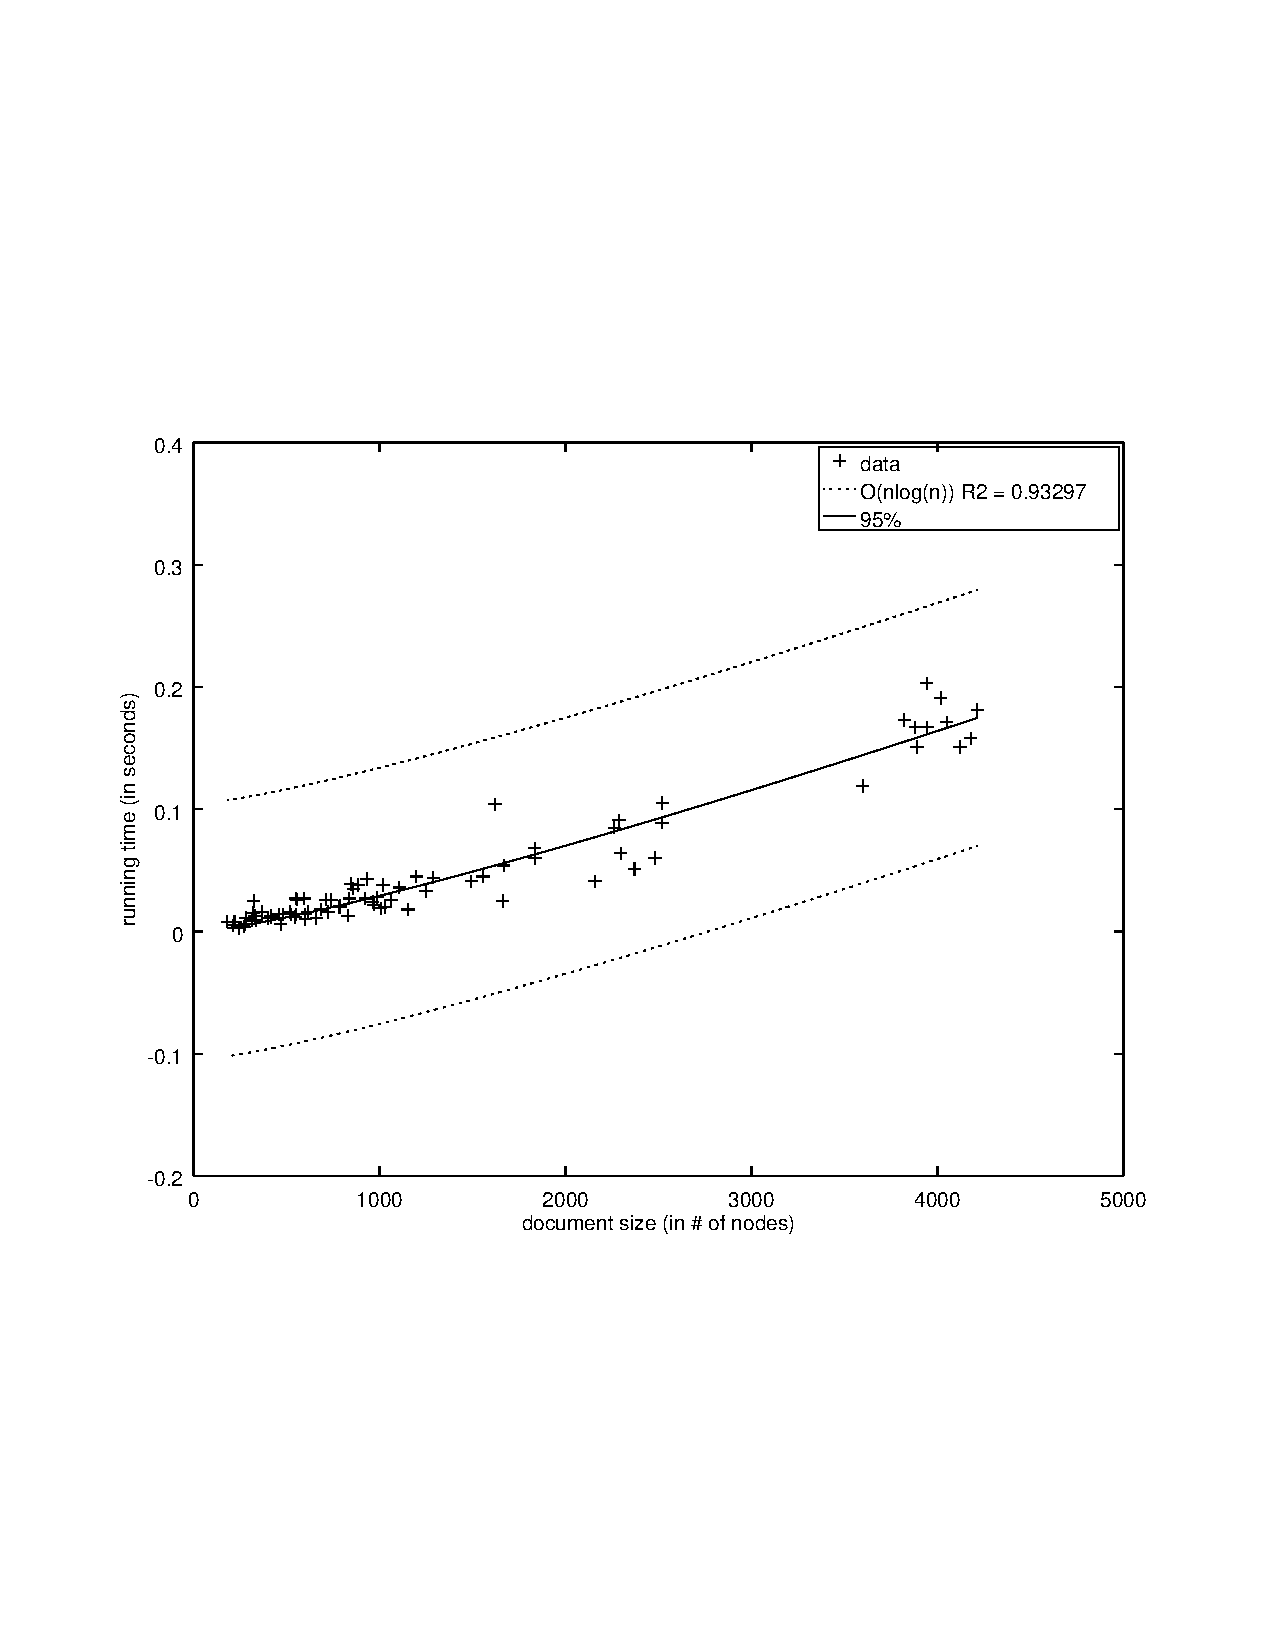
\includegraphics[trim={2.5cm 7.5cm 1cm 6.5cm}, width=\linewidth
     ]{img/runtime.pdf}
  \caption{Document size vs running time and rendering vs no rendering for all
  three datasets.}
  \label{fig:runtime}
\end{figure}

\section{Conclusion and Future Work}\label{sec:con}

We have shown here a novel approach for the problem of extracting records from
semi-structured web pages based on a new insight: seeing the structure of the
document as a cyclic signal. Our results are equivalent to the state-of-the-art,
but we claim we've achieved it in a more efficient way since no document
rendering is required. The structure detection in our approach can also be used
in other areas, for example, when the target is unstructured data one can rule
out structured noise (e.g., menus and advertising).

Although the high efficiency and effectiveness of our technique are demonstrated
by the results in Section \ref{sec:result}, it is not an error free approach.
We've assumed the records in a web document are contiguous, consistently
formatted / structured and with approximate size. Although these assumptions are
plausible, they are not universal and where they do not hold our approach fails.
Nonetheless, when considering web scale data, this subset of all structured data
is of considerable size and value.

In our opinion, the major set backs in this area of research are the
unavailability of implementations and the absence of a common framework.
Without the implementation of a particular technique we can't analyse individual
results to gain insight about why it did or did not work in a particular case.
This kind of analysis speeds up research because it helps refine research
assumptions faster, using previous works. On the other hand, a common framework
for the implementation of extractors reduces the variables involved in a
comparison by standardizing the basic software infrastructure (e.g., same HTML
parser used by everyone, same rendering engine, datasets, etc.). This problems
were pointed out in \cite{survey2013,survey2014} and would be mitigated by such
a framework.
 
Our guidelines for future work are the following:
\begin{enumerate}
  \item research alignment techniques: here we have used a general purpose and
  supralinear (but still polynomial) sequence alignment algorithm, but we
  believe it is possible to devise a solution specifically for the problem of
  record alignment that is more effective and has a lower complexity bound. In
  \cite{gfrerer2017parallel} a parallel approach is proposed;
  \item standardize datasets: the ideal testbed should consist of several
  randomly taken samples from a large scale search engine index with annotated
  ground truth.
  Such a dataset would enable the researcher to draw consistent conclusions
  from statistics (e.g., percentage of documents with structured content,
  ``real'' precision and recall). We haven't found such a dataset in the
  literature (i.e., one that is annotated for record extraction). With reliable
  statistics the amount of this kind of structured information could be
  correctly estimated, similar to what was done in \cite{webtables2008};
  \item use Goertezel's \cite{goertzel1958algorithm} in place of FFT:
  Goertezel's algorithm computes a single coefficient in linear time whereas the
  FFT computes all coefficients in linearithmic time. Our technique searches for a
  candidate frequency in a small range of the spectrum, there is no need to
  compute, up front, all coefficients so that may be an alternative to reduce
  the time complexity a little more;
  \item investigate the use of Lempel-Ziv\cite{ziv1977universal} (LZ) in the
  context of pattern detection: LZ is a computationally efficient compression
  algorithm targeted specifically at sequences, it works by looking for
  redundancies in the sequence, the redundancy (i.e., repeated data) can be seen
  as a recurring pattern (like contiguous records). We believe it is
  possible to exploit this algorithm in this context.
  %\item develop the extraction framework further: continue the development of
  %the extraction framework, refine and refactor code, implement other
  % extraction techniques, etc.
\end{enumerate}

%\appendix
%\section{Extraction Framework Usage Example}\label{app:a}

%Listing \ref{lst:lua} shows a small code snippet that parses an HTML document,
%extracts and displays the records found in it. The classes \texttt{DOM} and
%\texttt{DSRE} are implemented in C++ and their interfaces are exposed under the
%Lua environment.

%\begin{lstlisting}[label=lst:lua,language={[5.2]Lua},
%caption={Example of Lua source code calling C++ exposed interfaces.}]
% extractFile = function(filename) -- loads and parses HTML into a DOM tree 
%  local dom = DOM.new(filename)

%  -- instantiates an extractor
%  local dsre = DSRE.new() 

%  -- sets z-score and CV thresholds
%  dsre:setMinZScore(minZScore)
%  dsre:setMinCV(minCV)

%  -- extract records
%  dsre:extract(dom)

%  local regions = dsre:regionCount()
  
%  -- iterates over regions
%  for i=1,regions do
%    local dr = dsre:getDataRegion(i-1)
%    local rows = dr:recordCount()
%    local cols = dr:recordSize()

%    -- iterates over current region's
%    -- rows and columns
%    for r=1,rows do  
%      local record = dr:getRecord(r-1)
%      for c=1,cols do
%        -- output field value
%        print(record[c]:toString())  
%      end
%    end
%  end
	
%  dsre:printTps()
%  dom:printHTML()
%end
%\end{lstlisting}